\section{Problema de Valor de Contorno}


A solução de um problema regido por um modelo matemático depende de informações ligadas ao contexto em que tal problema ocorre.
Estas informações podem dizer a respeito das condições iniciais ou das condições de contorno. 
Condições iniciais caracterizam um Problema de Valor Inicial (PVI) e geralmente são relativas ao instante de tempo inicial do processo.
As condições de contorno por sua vez, caracterizam um Problema de Valor de Contorno (PVC) e  normalmente são dadas em função do limite espacial do processo em questão.
\citep[p. 447]{boyce_diprima}
Desta forma, enquanto os PVI geralmente relatam processos transientes, isto é, variantes no tempo, os PVC lidam com problemas em estado estacionário.

O PVI de um modelo de ordem $N$ é composto da equação do processo e do valor inicial da variável dependente e de suas derivadas, até a ordem $N-1$, como mostra a equação a seguir:

\begin{equation}
	\begin{cases}
		y'' + p(t)y' + q(t)y = f(t) \\
		y(t_0) = y_0 \\
		y'(t_0) = y_0'
	\end{cases}
\end{equation}

De forma análoga, o PVC é definido a partir da equação que modela o processo e suas condições nos pontos de contorno ou borda.

\begin{equation}
	\begin{cases}
		y'' + p(x)y' + q(x)y = f(x) \\
		y(x_i) = \alpha \\
		y'(x_f) = \beta
	\end{cases}
\end{equation}

Portanto, se as condições adicionais forem dadas em um único instante (ou ponto), tem-se o PVI do processo. Caso sejam dadas em dois ou mais pontos distintos, tem-se o PVC.

As condições de contorno usualmente podem ser classificadas como condições de Dirichlet ou de Neumann. 
As condições de Dirichlet são também conhecidas como essenciais e são estabelecidas sobre a variável dependente. Já as condições de Neumann são condições naturais e são impostas sobre a derivada a variável dependente. A seguir são dados alguns exemplos.

\begin{equation}
	\begin{tabular}{l l}
		$y(x_k) = y_k $ 
		& Cond. Dirichlet \\
		$y(x_k) = 0$
		& Cond. Dirichlet Homogênea\  \\
		$y'(x_k) = y_k$
		& Cond. Neumann \\
		$y'(x_k) = 0$
		& Cond. Neumann Homogênea\  \\
	\end{tabular}
\end{equation}




Dado o domínio $ \Omega $ tal que

\begin{equation}
  \Omega \subset \Re^{n}
\end{equation}

Os valores na fronteira $ \partial \Omega $ do domínio são definidos por uma função $ u(x, y) $ tal que

\begin{equation}
  u(x, y) = f(x, y),  \forall (x, y) \in \partial \Omega
\end{equation}

Assim, conhecendo-se os valores na borda, é possível inferir o conjunto de funções em $ \Omega $ que seja solução do modelo. 

De forma a exemplificar, considere o caso simples, em que o domínio $ \Omega $ seja um intervalo aberto em $ \Re $ e os pontos da fronteira sejam os extremos deste intervalo: 

\begin{equation}
  [a, b] \subset \Re
\end{equation}

\begin{equation}
  \Omega = [a, b]
\end{equation}

\begin{equation}
  \partial [a, b] = \{ a, b \}
\end{equation}

Um problema de valor de contorno definido sobre este domínio é portanto, composto pela equação que modela o comportamento do processo e pelas condições adicionais de contorno


\begin{equation}
    \label{eq:pvc}
    PVC : 
    \begin{cases}
        y'' = f(x, y, y') \\
        y(a) = \alpha \\
        y(b) = \beta
    \end{cases}
\end{equation}

Conforme mostra a figura ~\ref{fig:pvc}, a solução para o exemplo dado, consiste em encontrar a curva ou o conjunto de curvas que obedeçam às condições de contorno.

\begin{figure}[ht!]
\centering
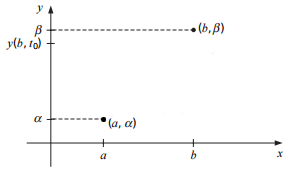
\includegraphics[scale=0.8]{figuras/PVC.png}
\caption{PVC: Encontrar a curva solução entre os pontos $ \alpha $ e $ \beta $}
\label{fig:pvc}
\end{figure}
